\chapter{Quantum Optimal Control Theory}
The fundamental problem of Quantum Optimal Control Theory is to steer the dynamics of a quantum system in a desired way through external fields \cite{Rice2000,Shapiro2003}. Often, the goal is the transfer from an initial state, $\ket{\psi_0}$, to the desired target-state, $\ket{\psi_{\mathrm{target}}}$. The fields responsible for controlling the dynamics of the system are parametrised by a set of control parameters or functions. Optimal control theory determines the parameters, which leads to the desired dynamics of the system \cite{Werschnik2007}.\\ 
In control problems, the Hamiltonian of the system is given as
\begin{equation}
	\hat{H} = \hat{H}_0 + \hat{H}_I = \hat{H}_0 + \sum_{n = 1}^{m} u_n(t) \hat{H}_n \; ,
	\label{eq:ControlHamiltonians}
\end{equation} 
where $\hat{H}_0$ is an uncontrollable drift of the Hamiltonian, $\hat{H}_i$ are the controllable fields, and $u_n(t)$ are the control functions or parameters. A quantum system like this is completely controllable if every unitary operator $\hat{U}$ is accessible from the identity operator $\hat{I}$ via a path $\gamma (t) = \hat{U}(t, t_0)$ satisfying \cite{Schirmer2001}
\begin{equation}
	i \partial_t \hat{U}(t, t_0) = \left( \hat{H}_0 + \hat{H}_I \right) \hat{U}(t, t_0) \; .
\end{equation} 
For an $N$-dimensional Hilbert spaces, a sufficient condition for complete controllability of a quantum system is that the Lie algebra generated by the Hamiltonians in eq. \eqref{eq:ControlHamiltonians},
\begin{equation}
	L_0 = \mathrm{Lie} \left( i \hat{H}_0, i \hat{H}_1 , \ldots , i \hat{H}_m \right) \; ,
\end{equation}
is of dimension $N^2$ \cite{Ramakrishna1995}.\\
Extending these conditions to infinite-dimensional Hilbert spaces and constrained controls is non-trivial \cite{Huang1983}. Therefore, no calculations of the Lie dimensions will be performed for the control problems presented in this thesis.


\section{The Gradient-Ascent Pulse Engineering Method}
In this instance, the control problem is steering an initial state to a target-state. More specifically, the transfer of a Superfluid to a Mott-Insulator, which is controlled by varying the lattice depth. Therefore, the optimal control problem can be stated as follows: 
Suppose the system is initially described by the state $\ket{\psi_0} = \ket{\psi (0)}$, and the potential is varied in the time interval $[ 0 , T]$. The goal is finding the set of control parameters, $\boldsymbol{u}(t)$, which brings the initial state as close as possible to the target state, $\ket{\psi_{\mathrm{target}}}$. This is formulated in terms of a cost function
\begin{equation}
	J_T = \frac{1}{2} \left( 1-|\braket{\psi_{\mathrm{target}} | \psi (T)}|^2 \right) \; ,
	\label{eq:infidelityCost}
\end{equation}
which is given as half the infidelity between the target and the state at $t=T$. The cost function becomes zero, when the terminal state matches the target state up to an arbitrary phase. Hence, the optimal control problem can be formulated as a minimization problem of eq. \eqref{eq:infidelityCost} \cite{Jager2014}.\\
Experimentally, large variations in the control parameter is often hard to achieve. Therefore, an extra term is often added to the cost function, which penalizes strong variations in the control. The new cost function reads
\begin{equation}
	J = J_T + \frac{\gamma}{2} \sum_{n=1}^{m} \int_{0}^{T} \left( \pdv{u_n}{t} \right)^2 \mathrm{d}t \; ,
	\label{eq:grapeCost}
\end{equation}
where $\gamma$ weighs the relative importance between matching states and smoothness of the control \cite{Jager2014}. As the state transfer is considered the highest priority, $\gamma$ is set as $\gamma \ll 1$, such that $J_T$ dominates the cost function of eq. \eqref{eq:grapeCost}.\\

A powerful way of performing optimal control is through the Gradient-Ascent Pulse Engineering (GRAPE) method. Through GRAPE, the gradient of the cost function \eqref{eq:grapeCost} can be evaluated and used to update the existing set of controls \cite{Khaneja2005}. Thereby, one achieves an optimization of the cost function.\\
The gradient of the cost function can be derived in multiple ways. A common method \cite{Hohenester2007, Winckel2008, BECcontrol} is introducing a Lagrange multiplier, which forces the dynamics to obey the Schrödinger equations. The derivation utilizes functional derivatives, as time, $\ket{\psi (t)}$, and the Lagrange multiplier are considered continuous functions. Later, the functions are discretized to perform numerical computations. Although this procedure is fairly easy, higher order correction terms of the gradient are absent due to the continuity of the functions.\\
Here, an alternative derivation following \cite{Khaneja2005, deFouquieres2011} is presented.

Assume the transfer time, $T$, is discretized in $M$ equal steps, $\Delta t = T/M$. Therefore, the control become similarly discretized as
\begin{equation}
	u_n = \left( u_n (t_1) , \ldots , u_n (t_M)  \right) \equiv \left( u_n (1) , \ldots , u_n (M)  \right) \; .
\end{equation}
Likewise, the time-evolution of the system during the time step $j$ is given by the propagator
\begin{equation}
	\hat{\mathcal{U}}_j \equiv \hat{\mathcal{U}} (u(t_j)) = \exp \lbrace -i \left(  \sum_{n = 1}^{m} u_n(j) \hat{H}_n  \right) \Delta t \rbrace \; . 
\end{equation} 
Thereby, the cost function \eqref{eq:grapeCost} becomes
\begin{equation}
	J = \frac{1}{2} \left( 1 - |\braket{\psi_{\mathrm{target}} | \prod_{j}^{M} \hat{\mathcal{U}}_j | \psi (0)}|^2 \right) + \frac{\gamma}{2} \sum_{n}^{m} \sum_{j}^{M-1} \left( \frac{\Delta u_n (j)}{\Delta t} \right)^2 \Delta t \; ,
	\label{eq:discreteCost}
\end{equation}
where $\Delta u_n (j) =  u_n (j+1) - u_n (j)$.\\
By defining $c \equiv \braket{\psi_{\mathrm{target}} | \psi (T)}$, the derivative with respect to the control of the first term of the discretized cost \eqref{eq:discreteCost} can be written as 
\begin{equation}
	\frac{\partial J_T}{\partial u_n (j)} = \frac{\partial}{\partial u_n (j)} \left( \frac{1}{2} |\braket{\psi_{\mathrm{target}} | \prod_{j}^{M} \hat{\mathcal{U}}_j | \psi (0)}|^2  \right) = \Re \left( c^* \frac{\partial c}{\partial u_n (j)} \right) \; .
	\label{eq:dJTdu}
\end{equation}
Focusing on $\frac{\partial c}{\partial u_n (j)}$ reveals
\begin{align}
	\frac{\partial c}{\partial u_n (j)} &= \frac{\partial }{\partial u_n (j)} \braket{\psi_{\mathrm{target}} | \prod_{j}^{M} \hat{\mathcal{U}}_j | \psi (0)} \nonumber \\
	&= \bra{\psi_{\mathrm{target}}} \hat{\mathcal{U}}_M \ldots \hat{\mathcal{U}}_{j+1} \frac{\partial \hat{\mathcal{U}}_{j}}{\partial u_n (j)} \hat{\mathcal{U}}_{j-1} \ldots \hat{\mathcal{U}}_{1} \ket{\psi (0)}
	\label{eq:dcdu}
\end{align}
Multiplying eq. \eqref{eq:dcdu} with $c^*$ to recreate the result of eq. \eqref{eq:dJTdu} yields
\begin{align}
	c^* \frac{\partial c}{\partial u_n (j)} &= \left( \braket{\psi(T) | \psi_{\mathrm{target}}} \bra{\psi_{\mathrm{target}}} \right) \prod_{j' = j +1}^{M} \hat{\mathcal{U}}_{j '} \frac{\partial \hat{\mathcal{U}}_{j}}{\partial u_n (j)} \prod_{j' = 1}^{ j-1} \hat{\mathcal{U}}_{j '} \ket{\psi (0)} \\
	&= -i \bra{\chi (T)} \prod_{j' = j +1}^{M} \hat{\mathcal{U}}_{j '} \frac{\partial \hat{\mathcal{U}}_{j}}{\partial u_n (j)} \prod_{j' = 1}^{ j-1} \hat{\mathcal{U}}_{j '} \ket{\psi (0)} \\
	&= -i \bra{\chi (t_j)}  \frac{\partial \hat{\mathcal{U}}_{j}}{\partial u_n (j)} \ket{\psi (t_{j-1})} \; ,
	\label{eq:gradientForBack}
\end{align}
where $\ket{\chi (T)} \equiv -i \ket{\psi_{\mathrm{target}}} \braket{\psi_{\mathrm{target}} | \psi (T)}$ is the projection of the final state unto the target state. Notice how in eq. \eqref{eq:gradientForBack} the state $\ket{\chi (T)}$ has been propagated backwards in time.\\ 
The derivative of the propagator, $\hat{\mathcal{U}}_{j}$, is non-trivial, due to the non-commutativity of the operators, $[ \hat{H}_0 \; , \; \hat{H}_n ]$. This results in a series of higher order corrections to the derivative.
Expressing the derivative as a Taylor series yields
\begin{align}
	\frac{\partial}{\partial u_n (j)} \left[ -i \hat{H} \Delta t \right] &= \sum_{p=1}^{\infty} \frac{ \left( -i \Delta t \right) ^p }{p!} \sum_{q=0}^{p-1} \hat{H}^k \hat{H}_n \hat{H}^{p-q-1} \nonumber \\
	&= \sum_{p=0}^{\infty} \sum_{q=0}^{\infty} \frac{A^p B A^q}{(p+q+1)!} \; ,
	\label{eq:derivTaylorExp}
\end{align}  
where $A = -i \hat{H} \Delta t$ and $B = -i \hat{H}_n \Delta t$. The factorial in the denominator can be split using
\begin{equation}
	\frac{1}{(p+q+1)!} = \frac{1}{p q !} \int_{0}^{1} (1-\alpha)^p \alpha^q \mathrm{d}\alpha \; ,
\end{equation}
whereby eq. \eqref{eq:derivTaylorExp} can be expressed as
\begin{equation}
	\sum_{p=0}^{\infty} \sum_{q=0}^{\infty} \frac{A^p B A^q}{(p+q+1)!} =  e^{A} \int_{0}^{1} e^{- \alpha A} B e^{ \alpha A} \mathrm{d}\alpha \; .
	\label{eq:doublesumToInt}
\end{equation}
Evaluating the resulting integral yields an iterative series of commutators
\begin{equation}
	\int_{0}^{1} e^{- \alpha A} B e^{ \alpha A} \mathrm{d}\alpha = \sum_{k=0}^{\infty} \frac{ (-1)^k}{(k+1)!} \left[ A \; , \; B \right]_k \; , 
	\label{eq:integralToComm}
\end{equation}
where $\left[ A \; , \; B \right]_k = \left[ A \; , \; \left[ A \; , \; B \right]_{k-1} \right]$ and $\left[ A \; , \; B \right]_0 = B$. This is otherwise known as the Baker–Campbell–Hausdorff expansion \cite{Wilcox1967}.\\
Combining equations \eqref{eq:derivTaylorExp}, \eqref{eq:doublesumToInt}, and \eqref{eq:integralToComm}, the derivative of the propagator can be written as the commutator series 
\begin{equation}
	\frac{\partial \hat{\mathcal{U}}_{j}}{\partial u_n (j)} = \exp \{ -i \hat{H} \Delta t \} \left( -i \hat{H}_n \Delta t + \frac{(\Delta t)^2}{2} \left[ \hat{H} , \hat{H}_n  \right] + \frac{i (\Delta t)^3}{6} \left[ \hat{H} , \left[ \hat{H} , \hat{H}_n  \right]  \right] - \ldots \right) \; .
	\label{eq:higherOrderGradient}
\end{equation}
For small time-steps the higher order corrections can be neglected, however, choosing a larger time-step reduces the run-time of the time-evolution, which is critical when describing many-body systems. Therefore, including higher order contributions increases the accuracy, whereby larger time-steps can be employed. Computing the higher order corrections can be done efficiently by analytically deriving the commutators beforehand. The increase in accuracy achieved depends on the system, as it is determined by the commutator $\left[ \hat{H} , \hat{H}_n  \right]$.\\
Lastly, combining equations \eqref{eq:dJTdu}, \eqref{eq:gradientForBack}, and \eqref{eq:higherOrderGradient} produces the final expression for the gradient of $J_T$ for the control at time $t_j$ 
\begin{equation}
		\frac{\partial J_T}{\partial u_n (j)}  = - \Re \left( \bra{\chi (t_j)} \hat{H}_n + \mathrm{h.o.}  \ket{\psi (t_{j})} \right)  \Delta t \; ,
\end{equation}
where $\mathrm{h.o.}$ denotes higher order terms described in eq. \eqref{eq:higherOrderGradient}.\\

The gradient of the cost function requires the computation of the regularisation term as well. The simplest approach is deriving the gradient from the continuous expression \eqref{eq:grapeCost} by taking the functional derivative
\begin{align}
	\frac{\delta }{\delta u_n (t')} \left[ \frac{\gamma}{2} \sum_{n=1}^{m} \int_{0}^{T} \left( \pdv{u_n}{t} \right)^2 \mathrm{d}t \right]
	&= \frac{\gamma}{2} \frac{\delta }{\delta u_n (t')} \left[ u_n \dot{u}_n \Big|_0^T - \int_0^T u_n \ddot{u}_n \mathrm{d}t \right] \nonumber \\
	&=  - \frac{\gamma}{2} \int_0^T \left( \pdv{u_n}{u_n (t')} \ddot{u}_n + u_n \pdv{\ddot{u}_n}{u_n (t')} \right) \mathrm{d}t  \nonumber \\
	&=  - \gamma \ddot{u}_n \; . \label{eq:regularisationGradient} 
\end{align} 
The continuous second derivative $\ddot{u}_n$ can easily be discretized for numerical calculations. Hence, the final expression for the cost gradient elements are given by
\begin{equation}
	\frac{\partial J}{\partial u_n (j)}  = - \Re \left( \bra{\chi (t_j)} ( \hat{H}_n + \mathrm{h.o.} )  \ket{\psi (t_{j})} \right)  \Delta t - \gamma \ddot{u}_n \; .
	\label{eq:costGradient}
\end{equation}\\

Through the analytically derived gradient, the cost can be iteratively updated using gradient-based optimization methods until a desired threshold is reached. This forms the framework of the Gradient-Ascent Pulse Engineering (GRAPE) algorithm \cite{Khaneja2005}, which is summarised below:

\begin{algorithm}
\begin{algorithmic}
\caption{GRAPE Algorithm}
\State Choose initial control $\boldsymbol{u}^{(1)}$.
\While{$ J > J_{\mathrm{threshold}}$}
	\State Calculate $\ket{\psi (t_k)} = \prod_{j=1}^{k} \hat{\mathcal{U}}_j \ket{\psi (0)}$ for $k = 1 \ldots M$.
	\State Calculate $\ket{\chi (t_k)} = \prod_{j=M}^{k} \hat{\mathcal{U}}_{j}^{\dag} \ket{\chi (T)}$ for $k = M \ldots 1$. 
	\State Evaluate $\frac{\partial J}{\partial u_n (k)}$ for $k = 1 \ldots M$ and $n = 1 \ldots m$ according to eq. \eqref{eq:costGradient}.
	\State Update controls using gradient such that $J^{(i + 1)} < J^{(i)}$. 
\EndWhile
\end{algorithmic}
\end{algorithm}
The computations are performed under the boundary conditions
\begin{align}
	\boldsymbol{u}(0) &= \text{fixed value} \\
	\boldsymbol{u}(T) &= \text{fixed value} \\
	\ket{\psi (0)} &= \ket{\psi_0} \\
	\ket{\chi (T)} &= -i \ket{\psi_{\mathrm{target}}} \braket{\psi_{\mathrm{target}} | \psi (T)} \; .
\end{align}
Figure \ref{fig:ControlUpdate} illustrates an update step of the controls such that the cost function is reduced.
\begin{figure}[!h]
	\centering
	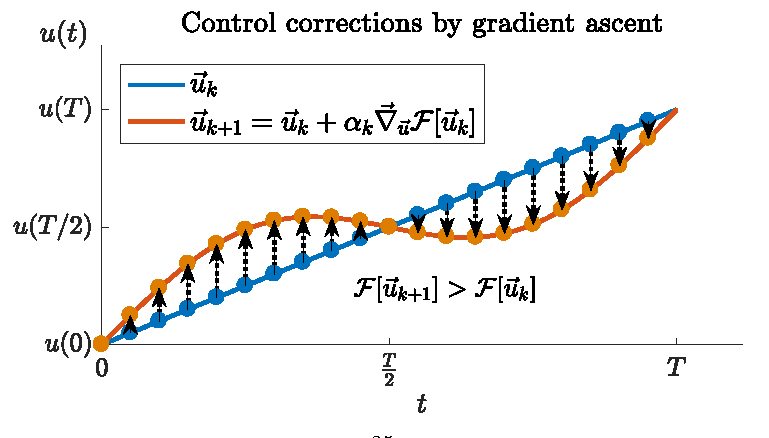
\includegraphics[width=0.7\columnwidth]{Figures/ControlUpdate.pdf} 
	\caption{ \textit{Visualisation of update step $i \to i+1$ the control $\boldsymbol{u}^{(i)}$ resulting in a decreased cost function.}}
	\label{fig:ControlUpdate} 
\end{figure} 
Although the starting guess of the control, $\boldsymbol{u}^{(1)}$, can be completely random, both faster convergence and lower convergence value is achieved by choosing a good starting seed. Clearly, there is no guarantee that the algorithm will converge to the global optimum, as it is based on a gradient ascent procedure \cite{Khaneja2005}. Nevertheless, the algorithm can be made to search a large portion of the parameter space by executing it multiple time for various seeds.  

\subsection{ $L^2$- vs. $H^1$-norm }


\section{Interior Point Method}
The convergence rate of the GRAPE algorithm has been shown to be greatly improved by employing gradient-based optimization methods for updating the control \cite{Jager2014}.
Interior point methods are modified versions of Newtons method for bound, constrained problems. The methods approach the solution from within the feasible region and provides efficient performance while having better theoretical properties than the standard simplex method \cite{wright}.\\

Here, a linear version of the method will be derived, however, the formalism can easily be extended to non-linear problems \cite{wright}.
Consider the general minimization problem
 \begin{align*}
	\min_{x \in \mathbb{R}^n} \;  & \; c^T x \\
	\text{subject to} \;  & \; A x = b  \\
							& \; x \geq 0 \; ,
\end{align*}
which can be derived from any linear problem through slack variables that transform inequality constraints into equality constraints at the cost of introducing extra variables \cite{ipopt}.

\subsection{Karush–Kuhn–Tucker conditions}
A central concept in mathematical optimization is the Karush–Kuhn–Tucker (KKT) conditions, which are first-order conditions for a solution of a nonlinear problem to be an optimum. The KKT conditions allow inequality constraints, whereby they are more general than Lagrange multipliers. 
\begin{theorem}
	Suppose that $x^*$ is a local solution of the objective function $f \; : \; \mathbb{R}^n \to \mathbb{R}$ with respect to a collection of constraints $\{ c_i(x)  \}_{i=1}^{m}$, where $c_i \; : \; \mathbb{R}^n \to \mathbb{R}$. Let $\mathcal{L}$ be the Lagrangian of the problem. If the subset of the equality constraints $\{ c_i(x) \in \mathcal{E}\}$ has the property that $\{ \nabla c_i(x^*)\}$ is linear independent, then a vector of Lagrange multipliers, $\lambda^*$, exists for which the following holds:
	\begin{subequations}	
	\begin{align}
		\nabla_x \mathcal{L}(x^*,\lambda^*) &= 0 \; ,  \\
		c_i(x^*) &= 0 \; , \qquad \forall i \\
		\lambda_{i}^* &\geq 0 \; , \qquad \forall i \in \mathcal{I} \\
		\lambda_{i}^* c_i(x^*) &= 0 \; , \qquad \forall i \in \mathcal{E} \cup \mathcal{I}
	\end{align}
	\end{subequations}	
	where $\mathcal{E}$ and $\mathcal{I}$ denote the equality and inequality subspaces respectively \cite{wright}.  
\end{theorem}
The KKT conditions is a way of determining, whether a point is an optimum. If $x^*$ satisfies the conditions, its objective value must be lower than the objective point of any other point.


\subsection{Barrier Problems}
In interior point methods the boundaries of the variables are enforced through a barrier function, which keeps the objective function continuously differentiable.
A general, linear optimization problem can be associated with a barrier function
\begin{equation}
	B(x , \mu) = c^T x - \mu \sum_{i=1}^{n} \ln x_i \; ,
\end{equation} 
where the barrier parameter $\mu > 0$. For $\mu \to 0$ one recovers the original problem.
The optimization Lagrangian of the barrier problem is
\begin{equation}
	\mathcal{L}(x, \lambda, s) = c^T x - \mu \sum_{i=1}^{n} \ln x_i - \lambda^T (A x -b) \; ,
\end{equation}
where $\lambda \in \mathbb{R}^m$ is the Lagrange multiplier for the $A x = b$ constraint. Now, let $X = \mathrm{Diag}(x_1 , \ldots , x_n)$, $e = (1,1, \ldots , 1)^T$, $s = \mu X^{-1} e$, and $S = \mathrm{Diag}(s_1 , \ldots , s_n)$. Thereby the KKT conditions of the barrier problem can be stated as 
\begin{subequations}
\begin{align}
	A^T \lambda + s &= c \\
	A x &= b \\
	X S e &= \mu e \; .
\end{align}
\end{subequations}
By adding the barrier term the KKT complementary condition has been "relaxed", as it is no longer equals zero \cite{ipnote}. Again, for $\mu \to 0$ the original conditions are recovered. 


\subsection{Primal-Dual Interior Point Method}
Primal-dual methods optimize an additional, \textit{dual}, problem while optimizing the main, \textit{primal}, problem.
Consider the initial linear problem. Its dual is defined as 
\begin{align*}
	\max_{\lambda \in \mathbb{R}^n} \;  & \; b^T \lambda \\
	\text{subject to} \;  & \; A^T \lambda + s = c  \\
							& \; s \geq 0 \; .
\end{align*}
If either the primal or the dual problem has a solution, then so does the other, and the objective values are equal. If either problem is unbounded, then the other problem is infeasible. If a solution exists, then the optimal solution to the dual problem are the Lagrange multipliers to the primal problem and vice versa \cite{wright}. Note, how the dual of the dual problem is the original problem.
Hence, for primal-dual algorithms triplet of variables, $(x , \lambda , s)$, is considered when computing the optimum of a function.\\

The primal-dual interior point method computes a constrained Newton step, which is used to iterate the variables towards the optimum. Thisis done by solving a primal-dual barrier problem for a given $\mu$, yielding the optimum solution of said subproblem. The optimal solution of the main problem is found by solving these subproblems iteratively for ever decreasing $\mu$ using the previous solution as starting point \cite{ipopt}.\\
The solutions for the primal-dual subproblems are characterized by the KKT conditions. These conditions can be written into a single mapping
 \begin{align}
    F(x , \lambda, s) &= \begin{pmatrix}
           A^T \lambda + s - c \\
           A x - b \\
           X S e
         \end{pmatrix} = 0
  \end{align}
  which has the Jacobian
 \begin{align}
    J(x , \lambda, s) = \begin{pmatrix}
           0 & A^T & I	\\
           A & 0 & 0 	\\
           S & 0 & X
         \end{pmatrix}
  \end{align}
Thus, the Newton direction, $(x_B , \lambda_B , s_B)$, can be written as the solution to the system of equations
\begin{align}
J \begin{pmatrix}
           x_B \\
           \lambda_B \\
           s_B
         \end{pmatrix} = -F
\end{align}
This equation does not take into account the barrier function, however, as stated earlier, the effect of the barrier term is to relax the the KKT complementary condition. This is achieved by setting $X S e = \mu e$, whereby one obtains
\begin{align}
	\begin{pmatrix}
    	 0 & A^T & I    \\
         A & 0 & 0 		\\
         S & 0 & X
    \end{pmatrix} 
    \begin{pmatrix}
    	x_b 		    \\
        \lambda_B		\\
        s_B
    \end{pmatrix} =
    - \begin{pmatrix}
    	  A^T \lambda + s - c 	\\
          A x - b 				\\
          X S e - \mu e
    \end{pmatrix} \; . \label{eq:newtondirection}
\end{align}
Thereby the parameters can be iteratively updated through the calculated Newton direction
\begin{equation}
	(x_{k+1} , \lambda_{k+1} , s _{k+1}) = (x_{k} , \lambda_{k} , s _{k}) + \alpha  (x_B , \lambda_B , s_B) \; , \label{eq:newtonstep}
\end{equation}
where $\alpha$ can be found using a line-search or other more sophisticated methods.
The procedure above can be summarized in the following algorithm \cite{ipnote}:\\
\begin{algorithm}
\begin{algorithmic}
\caption{Primal-Dual Interior Point Algorithm}
\State Choose $\sigma \in (0,1)$ and $\mu_0 > 0$.
\State Choose initial point $(x_0 , \lambda_0 , s_0)$ within feasible region.
\For{$k = 1 , \ldots$}
	\State $\mu_k \gets \sigma \mu_{k-1}$
	\State Calculate the Newton direction using eq. \eqref{eq:newtondirection}.
	\State Compute step-size $\alpha$.
	\State Update parameters according to eq. \eqref{eq:newtonstep}
\EndFor
\end{algorithmic}
\end{algorithm}


\section{Quantum Speed Limit}
A subtlety of optimal control problems is that one is only searching for the control, $\boldsymbol{u}(t)$, which steers the initial state into the target-state at time $t = T$. It is often desirable to obtain the desired state in the shortest timespan possible. However, if a solution exists at $t= T_1$, it might not exist at $t = T_2 < T_1$. The shortest duration for which a solution can be found is called the \textit{quantum speed limit} (QSL). A large energy difference to orthogonal states allows for fast oscillations within a system, however, these differences cannot be arbitrarily large. Hence, a lower bound of how fast a system can evolve exists, which in turn leads to the QSL \cite{Caneva2009}.\\
There are several ways of approximating the quantum speed limit, however, there is no known way to reliably determine the QSL for a general state. Therefore, the best option is often to just solve the problem at increasingly shorter durations, until a solution no longer can be found [JJ].\\
If the initial state, $\ket{\psi_0}$, and the target-state, $\ket{\psi_{\mathrm{target}}}$, are orthogonal, one can estimate the QSL from the orthogonalization time, which is how long it takes for a state to become orthogonal to itself.
Consider $\ket{\psi (0)} = \sum_{n}^{\infty} c_n \ket{\phi _n}$, where $\hat{H} \ket{\phi _n} = E_n \ket{\phi _n}$. Following \cite{QSLtoffoli}, the norm squared of the survival probability is given as
\begin{align}
	|S(t)|^2 = |\braket{\psi (0) | \psi (t)}|^2 &= \sum_{n , m = 0}^{\infty} |c_n|^2 |c_m|^2 \cos \left( (E_n - E_m) t \right) \nonumber \\
	&\geq 1 + \frac{4 t}{\pi ^2} \dv{|S(t)|^2}{t} - \frac{4 t^2}{\pi} \Delta E^2 \; ,
\end{align}
where the trigonometric inequality $\cos x \geq 1 - \left( 4 x \sin x - 2 x^2 \right) / \pi^2$ was used, and $\Delta E$ is the energy spread of the state.
Since $|S(t)|^2 \geq 0$, then $\dv{|S(t)|^2}{t} = 0$ whenever $|S(t)| = 0$, which is the case at the orthogonalization time $t = \tau$. This leaves the inequality $0 \geq 1 - 4 \tau^2 \Delta E^2 / \pi^2$, yielding the Mandelstram Tamm bound when solved \cite{Mandelstam1991}
\begin{equation}
	\tau_{\mathrm{MT}} \geq \frac{\pi}{2 \Delta E} \; .
	\label{eq:MandelstamBound}
\end{equation}
Eq. \eqref{eq:MandelstamBound} sets a lower bound of the orthogonalization time, however, the bound was derived using a constant Hamiltonian. In the case of optimal control, the Hamiltonian is time dependent, which can be taken into account by using arguments from differential geometry \cite{Aharonov,beyondQSL}
\begin{equation}
	\tau_{\mathrm{MT}} \geq \frac{\pi}{2} \left( \int_{0}^{T} \Delta E \; \mathrm{d}t \right) ^{-1} \; , \label{eq:MTlimit}
\end{equation}
Equations \eqref{eq:MandelstamBound} and \eqref{eq:MTlimit} show how fast solutions require a large value of $\Delta E$. Since \ref{eq:MTlimit} is dependent on the control $\boldsymbol{u}(t)$, one would have to take an infimum over all controls connecting the initial and target state in order to evaluate the lowest value of the bound. This in itself is a task just as difficult as solving the control problem.